\documentclass[12pt,a4paper]{article}
\usepackage[utf8]{inputenc}
\usepackage[spanish]{babel}
\usepackage{amsmath}
\usepackage{amsfonts}
\usepackage{amssymb}
\usepackage{makeidx}
\usepackage{graphicx}
\usepackage[left=2cm,right=2cm,top=2cm,bottom=2cm]{geometry}
\usepackage{multicol}
\usepackage{float}
\usepackage{wrapfig}
\raggedcolumns
\begin{document}
\begin{titlepage}

\centering

\includegraphics[scale=0.3]{UNC.PNG}

\vspace{1cm}
{\bfseries\LARGE Universidad Nacional de Córdoba \par}
\vspace{1cm}
{\scshape\Large Facultad de Matemática, Astronomía, Física y Computación\par}
\vspace{1cm}
{\scshape\Huge Trabajo Práctico N°3 de Redes Neuronales}
\vspace{1cm}

{\Large Chediack Ciminari, Camila }
\vspace*{0.3cm}


DNI: 41919762 \\


\vspace*{0.3cm}

E-mail:camila.chediack.c@mi.unc.edu.ar

\end{titlepage}
\begin{multicols}{2}
\begin{center}
\begin{large}
\textbf{Introducción}
\end{large}
\end{center}
\bigskip

En el presente informe se aplica una red feed-forward auto-encoder, con una capa oculta, a la base de datos de Fashion-MNIST, la cual consiste en un conjunto de imágenes de prendas y calzados clasificados en 10 categorías. 

Las redes neuronales feed-forward estan compuestas por \textit{N} capas donde \textit{N-1} estan ocultas. Esta convención no contabiliza la primer capa de neuronas, sino que esta representa el \textit{input} de  la red. La particularidad que tiene este tipo de redes es que las conexiones se realizan entre las unidades de una capa y la inmediatamente posterior, no hay conexiones entre las unidades de una misma capa ni entre estas y capas anteriores o dos capas más adelante. En la \textbf{Figura N°1} tenemos el ejemplo de un perceptrón simple:

\begin{center}
\textbf{Figura N°1: Red Feed-Forward}
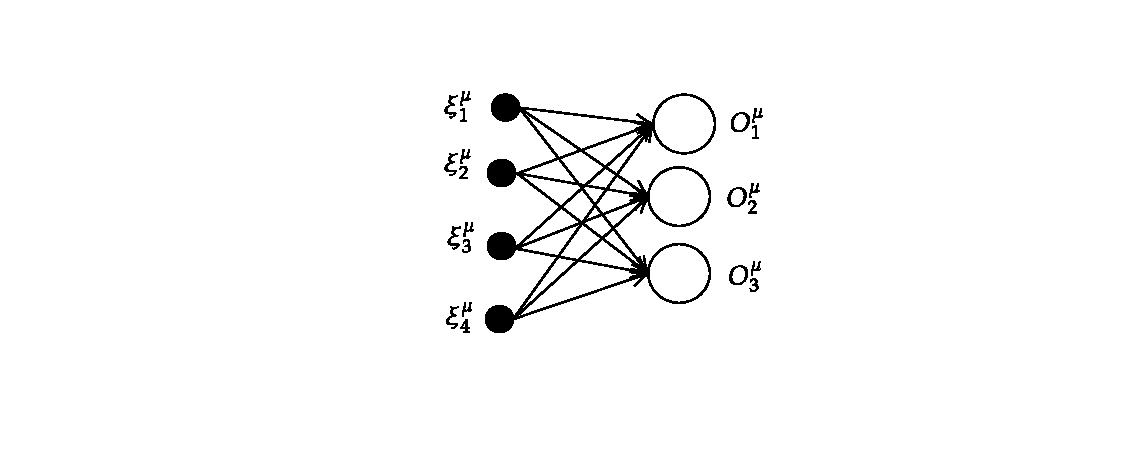
\includegraphics[scale=0.45]{red.pdf}
\end{center}


Que puede computarse a través de la siguiente función:

\begin{equation}
O^{\mu}_i = g(h_i) = g(\sum_k w_{ik} \xi_k)
\end{equation}

Como se denota en la ecuación (1), la relación o conexiones entre las neuronas de entrada y las neuronas de salida se representan a través de los ponderadores $w_{ik}$, donde el subíndice $k$ hace alusión a la neurona de entrada e $i$ a la neurona de salida. El cálculo de estos ``ponderadores'' va a depender del tipo de Red Neuronal que se utilice y de los parámetros que se especifiquen. 

En este caso al utilizarse una red feed-forward autoencoder, tiene la particularidad que la capa de entrada y la capa de salida deben tener la misma cantidad de neuronas, mientras que las capas intermedias deben tener una cantidad menor de neuronas. Esto obliga a la red a encontrar patrones entre los elementos, de forma que aprenda a presentar la información comprimida y permitiendo así reducir la dimensionalidad de los datos. En nuestro caso al trabajar con una sola capa oculta, obtendríamos lo que se ve en la \textbf{Figura N°2}.

\begin{center}
\textbf{Figura N°2: Autoencoder}
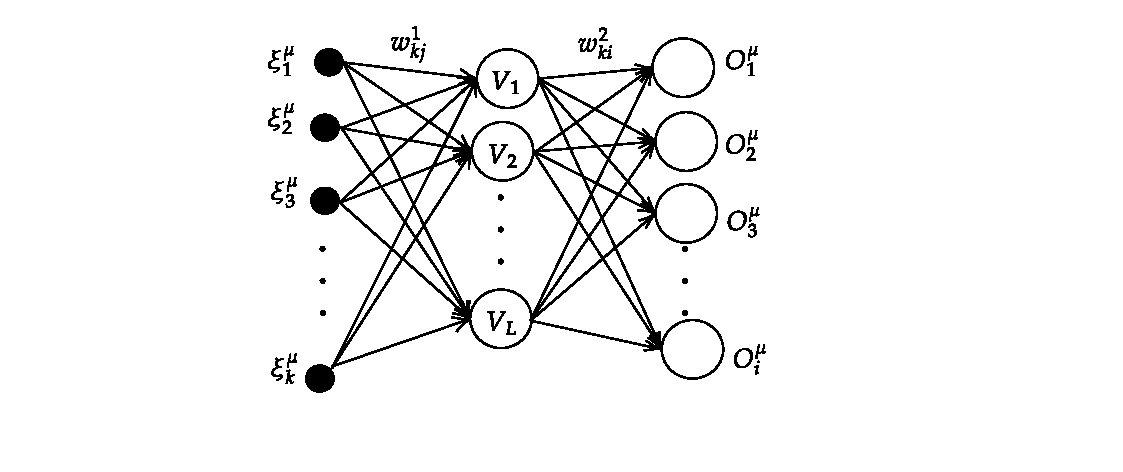
\includegraphics[scale=0.5]{red1.pdf}
\end{center}

\begin{center}
\begin{large}
\textbf{Modelo de Red Neuronal}
\end{large}
\end{center}

En esta sección se explicará con mayor nivel de detalle cuestiones a fines del armado de la arquitectura de una red neuronal.

Tras haber definido la cantidad de capas de la red neuronal se debe elegir la función de activación adecuada, siendo que esta es muy importante para el buen funcionamiento del modelo. Las redes neuronales aprenden de sus errores, a esto se lo denomina retropropagación del error (\textit{backpropagation}) y consiste en hacer una suma ponderada de las entradas a través de la \textit{función de activación} con el fin de obtener un valor de predicción. La diferencia entre este resultado y la predicción esperada es el ``error de predicción'', que una vez obtenido, se recorre la neurona en sentido inverso para considerar el error cometido durante la predicción y asi ajustar los valores de los pesos sinápticos (o ponderadores). 

En este caso se va a elegir ReLU como función de activación, esta actúa anulando los números negativos y dejando a los positivos sin modificaciones, dejando de lado el problema de desaparición del gradiente. Se va a utilizar un dropout $p = 0.1$, esto significa que con una probabilidad igual a $p$ y de forma aleatoria, va a convertir en cero algunos elementos de la entrada,  esto mejora el desempeño de la red neuronal evitando o disminuyendo la posibilidad de \textit{overfiting}. 

Como función de pérdida se va a utilizar el error cuadrático medio y el método del descenso por el gradiente estocástico como algoritmo para minimizar dicha función, con una tasa de aprendizaje (\textit{learning-rate}) que indica ``de que tamaño'' dar el paso para que el algoritmo converga a la solución. Lo ideal es hacerlo de forma proporcional al gradiente, en caso de descender mucho si la función crece mucho y descender poco si la función crece poco.

Establecer su valor ``óptimo'' no es tan sencillo, un valor muy pequeño puede provocar que el gradiente quede atrapado en un mínimo local y que por ende no actualice bien el cálculo de los ponderadores (es decir, la función no se estaría minimizando de forma correcta). Por otro lado, si se establece un valor muy alto, el gradiente puede pasar de largo el mínimo global y nunca encontrarlo, a pesar de que el apredizaje sea más rápido. 

Seguidamente a la hora de entrenar la red neuronal se deben elegir los valores que van a asumir los otros \textbf{hiperparámetros}, en esta caso se va a elegir un minibatch de tamaño 1000 y se va a entrenar por 200 épocas. 

El proceso del descenso por el gradiente se puede hacer por \textbf{batch}, es decir que, se calcula el error para cada muestra pero actualiza el modelo después de entrenar todas las muestras. Cuando el descenso por el gradiente es estocástico, se calcula el error y se actualiza el modelo por cada muestra, como si se estuviera trabajando con batch de tamaño igual a 1 (60 mil muestras). Por último, el método que se va a implementar en esta caso es con minibatch, donde se utiliza una pequeña porción de los datos como batch, por cada mil muestras se calcula el error y se actualiza el modelo, en total vamos a tener 60 batchs. A su vez, este procedimiento se va a repetir por cada una de las épocas. 

\begin{center}
\begin{large}
\textbf{Red feed-forward auto-encoder sobre Fashion-MNIST}
\end{large}
\end{center}

Al tratarse de un Autoencoder ``simple'' y no un clasificador, lo que se busca es entrenar a la red neuronal para que pueda reconstruir las distintas imágenes proveidas por la base de datos Fashion-MNIST, compuesta por un conjunto de entrenamiento de 60 mil imágenes y un conjunto de testeo de 10 mil imágenes de 28x28 (784 en total) píxeles en escala de grises. Cada una de ellas se encuentra asociada a una etiqueta, la cual no va a ser relevante en este caso ya que solo se va a entrenar el modelo para que devuelva la imagen.  

La red neuronal a implementar va a tener como datos de entrada 784 neuronas (una por cada pixel de la imagen) y \textit{una sola capa intermedia} que va a ir variando de tamaño: $n = 64, 128, 256 \ y \ 512$. Los datos de salida tienen que ser del mismo tamaño que los datos de entrada, el propósito es entrenar las neuronas a partir de la función identidad, primero codificando a información reduciendo el número de neuronas y volviendo a decodificar la información hasta que las neuronas de salida cuenten con el mismo número de neuronas a la entrada. 

La red va a aprender a partir del conjunto de entrenamiento, mientras que el conjunto de testeo se va a utilizar para corroborar que las predicciones del modelo sean correctas y que cuando se tome un imagen de dicho conjunto la red reconozca que tipo de prenda a través de la reconstrucción de su imagen.

\begin{center}
\begin{large}
\textbf{Resultados}
\end{large}
\end{center}

A continuación se muestra la gráfica de las funciones de pérdida sobre el conjunto de entrenamiento y sobre el de testeo, estas funciones nos dan una pauta sobre el desempeño de la red.

\begin{center}
\textbf{Figura N°5: Funciones de pérdida}
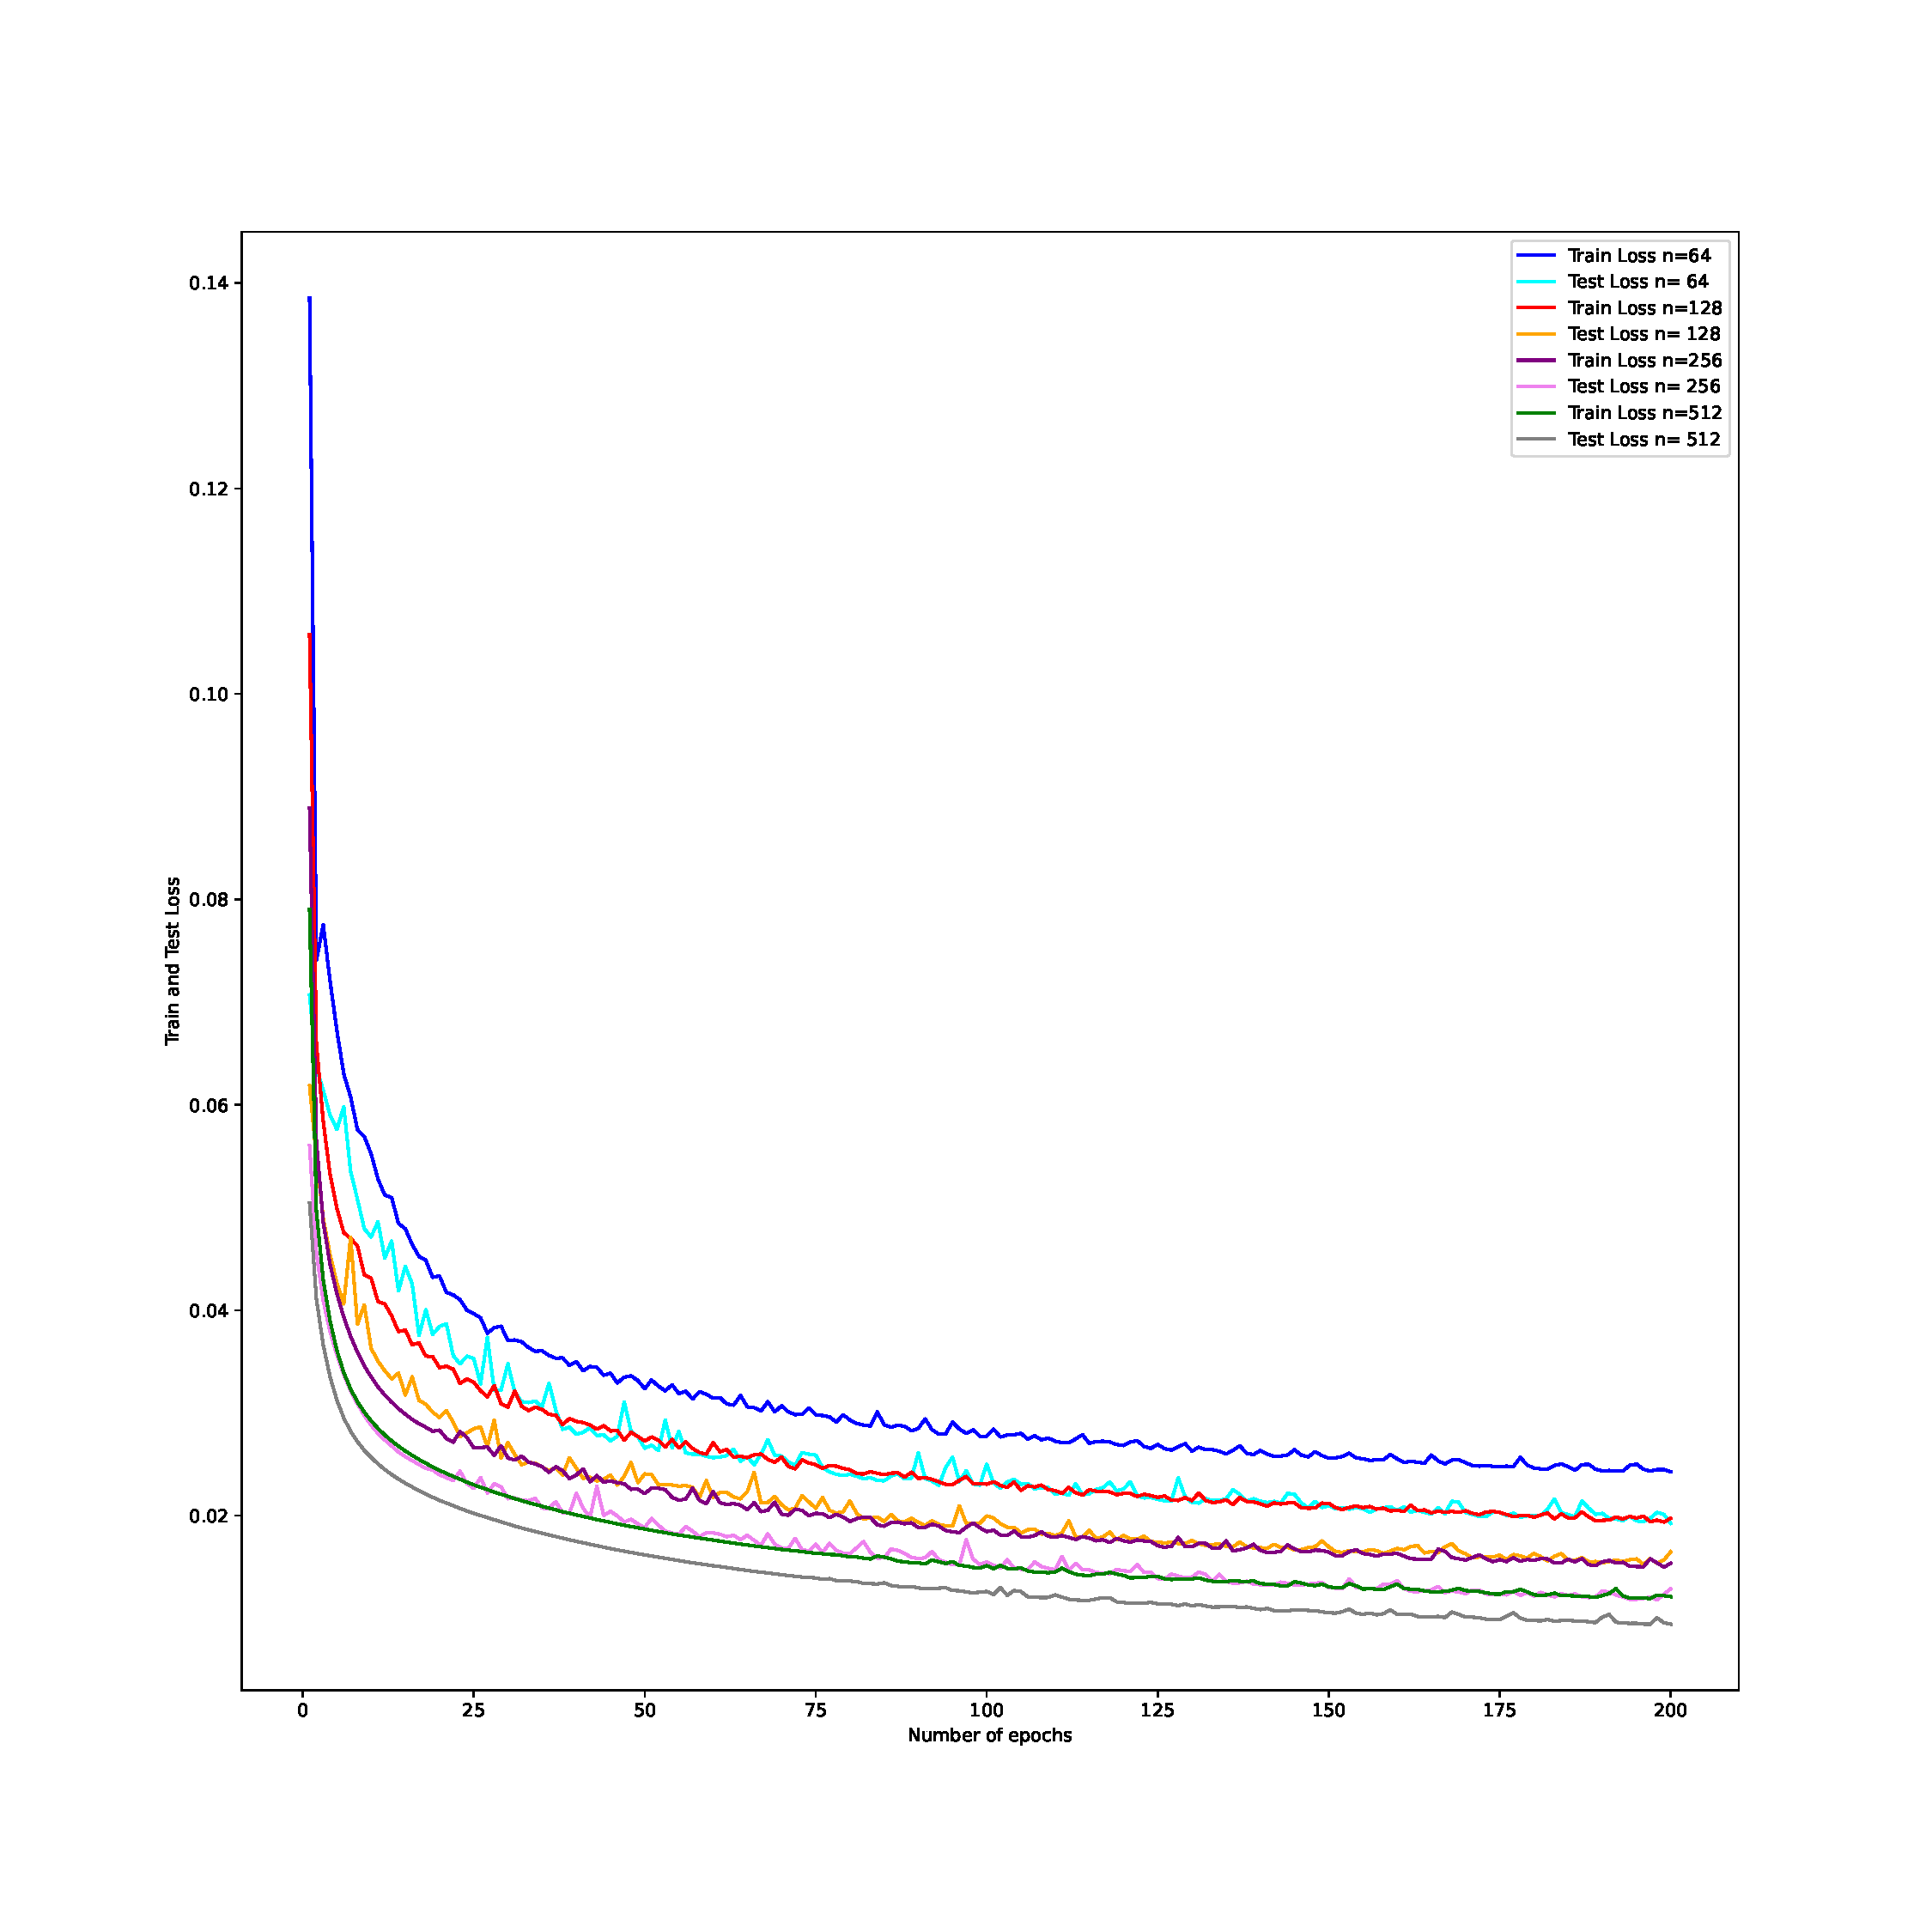
\includegraphics[scale=0.22]{Loss.pdf}
\end{center}

En todos los casos la función de pérdida del conjunto de entrenamiento se encuentre por encima de la función de testeo nos da una buena señal de que la red aprendió bien del conjunto de entrenamiento y que no ocurrió un \textit{overfiting}, estos datos son conocidos y si bien la red no aprende al 100\% de ellos (por eso calculamos también el error de entrenamiento) si debería haber un buen ajuste de los datos, es por ello que se vuelve fundamental probar el desempeño del modelo sobre datos desconocidos y ver si el modelo los predice de forma correcta. Al comparar distintos modelos entramos en un trade-off entre elegir aquel modelo que no solo se ajuste bien al conjunto de entrenamiento sino que también funcione correctamente para predecir sobre el conjunto de testeo, siendo preferible uno \textbf{extrapola mejor} a uno que tiene mejor ajuste del conjunto de entrenamiento.

\begin{center}
\textbf{Figura N°3: Funciones de pérdida del conjunto de entrenamiento}
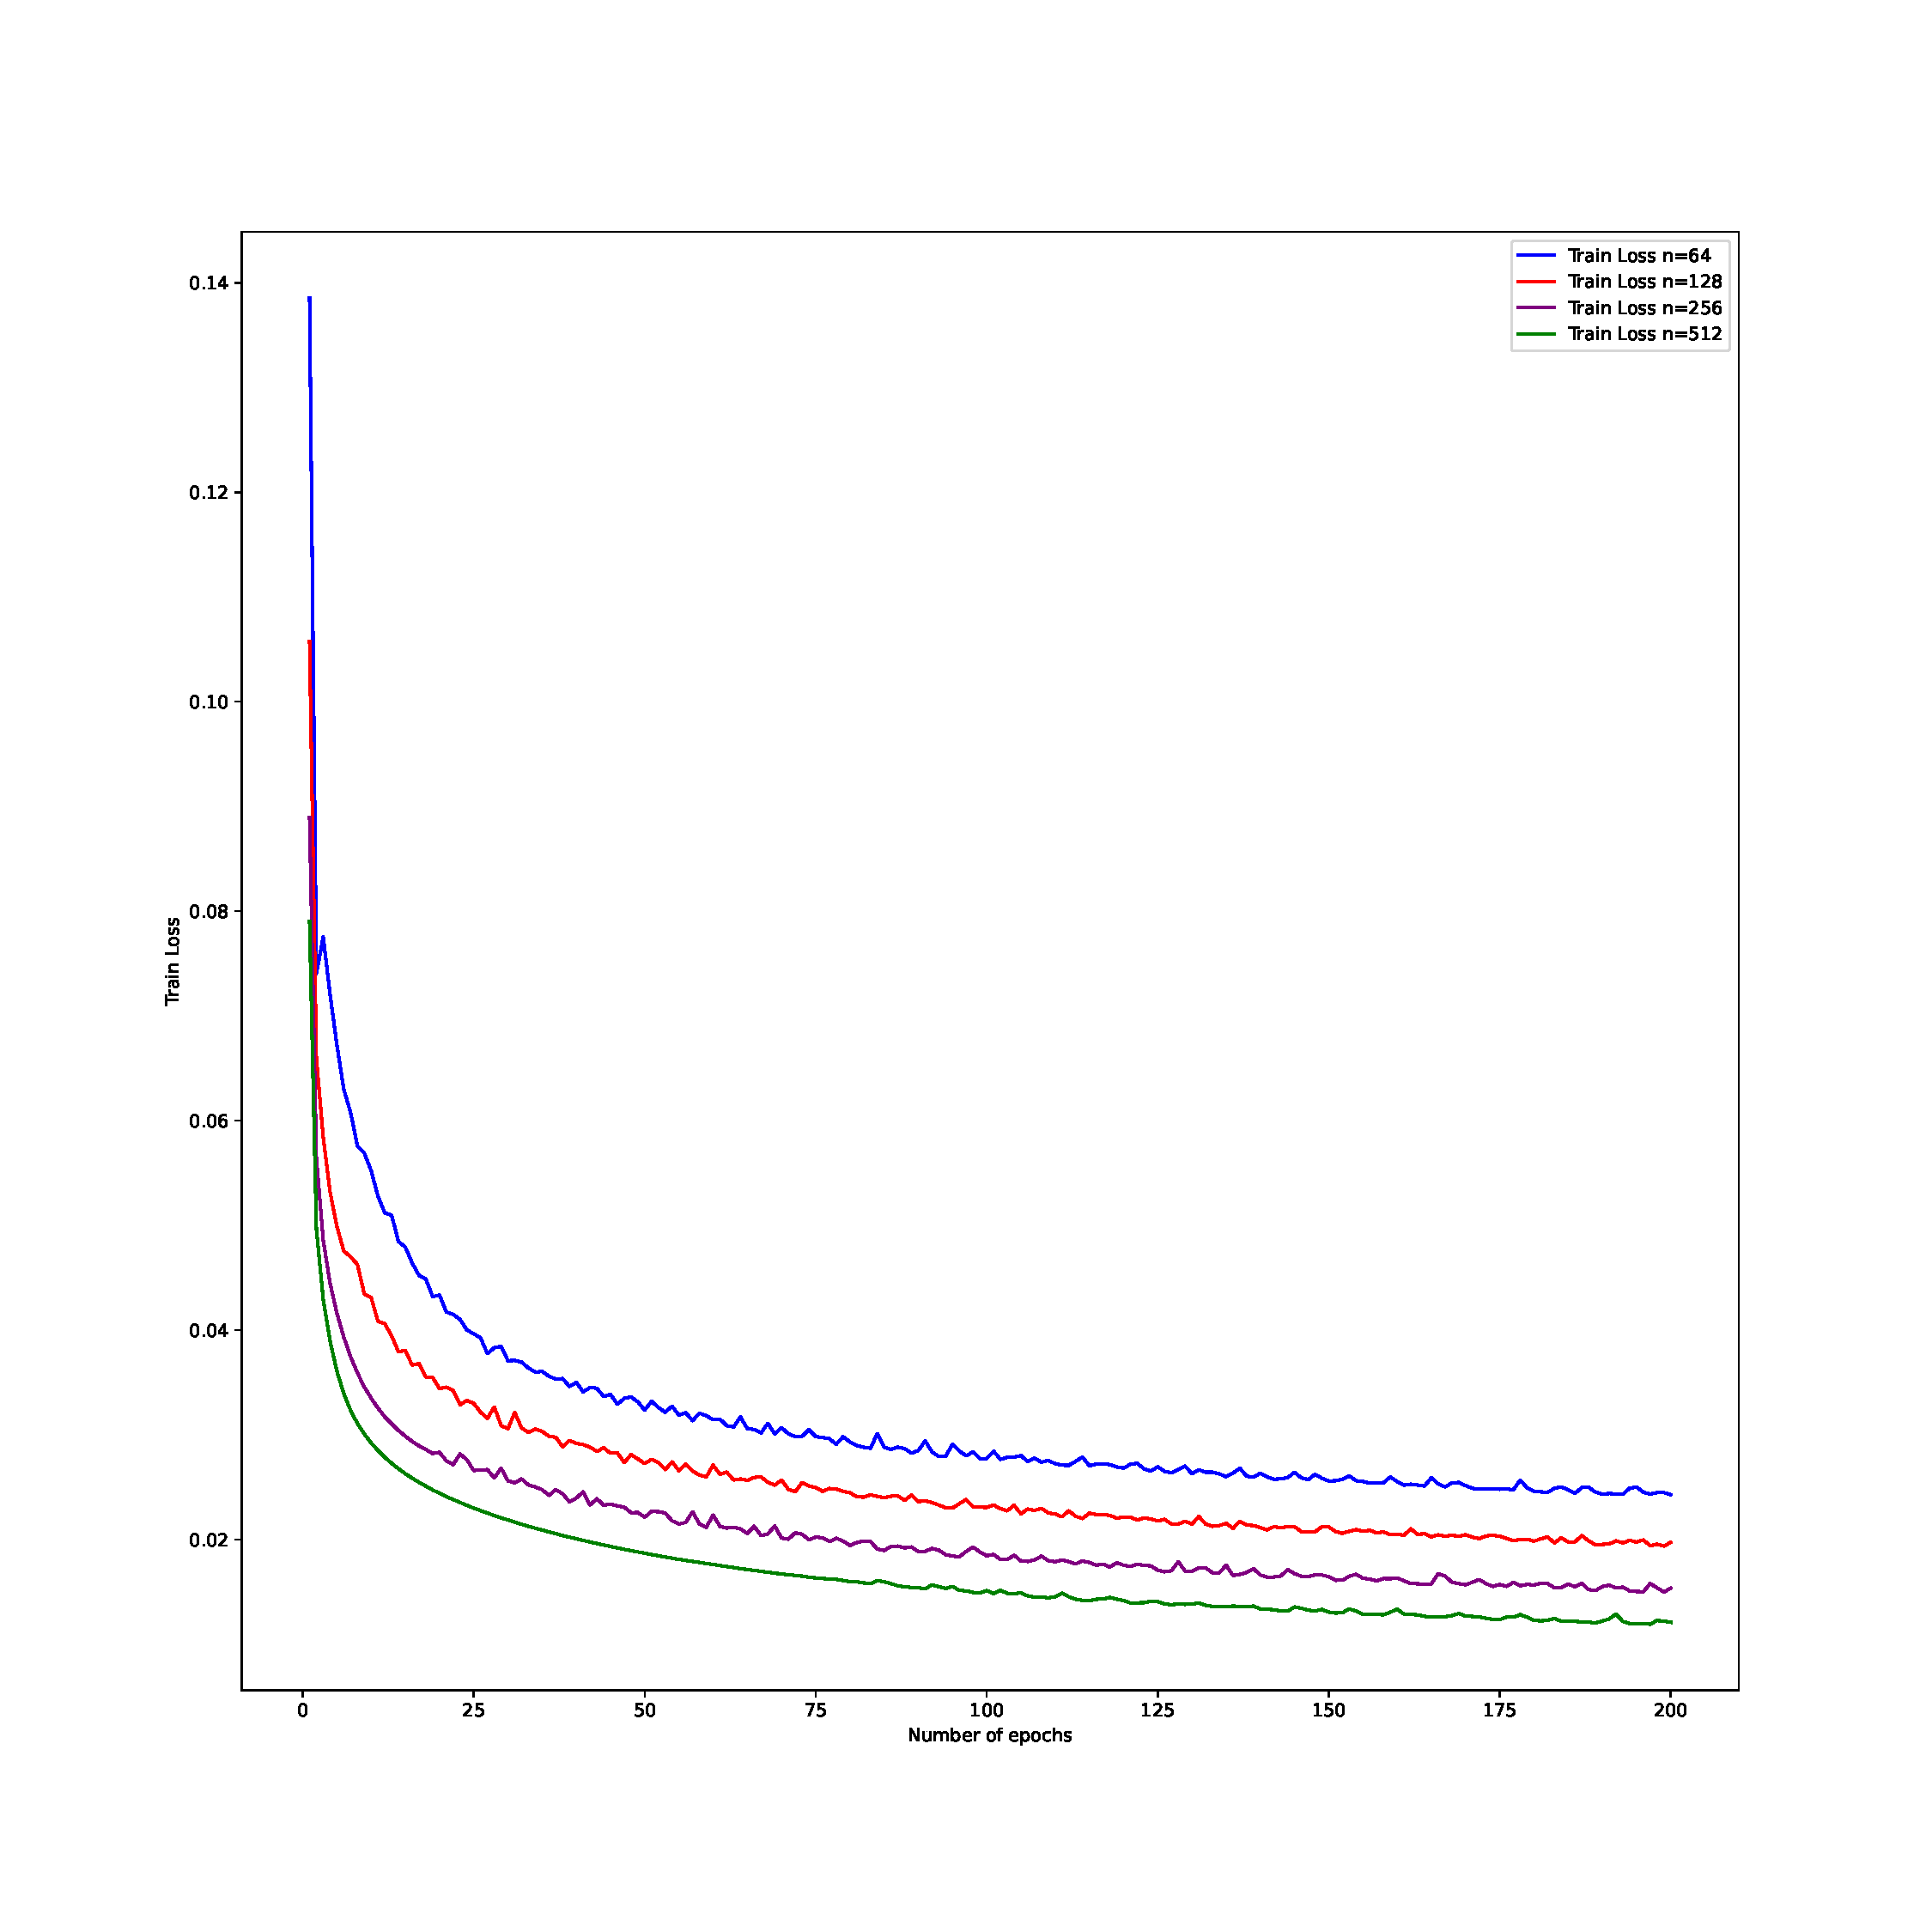
\includegraphics[scale=0.20]{Train Loss.pdf}
\end{center}

Mientras mayor es el tamaño de la capa intermedia menor valor asume la función de pérdida sobre el conjunto de entrenamiento, pasando las primeras épocas, en un principio vemos que algunas se superponen entre sí. Esto en parte se debe a qu la reducción de dimensionalidad de los datos es menor y no se pierde tanta información al pasar de 784 a 512 neuronas. 

En las funciones de pérdida para el conjunto de testeo se presenta el mismo patrón en el que el error disminuye con el aumento del tamaño de capa intermedia. 

\begin{center}
\textbf{Figura N°4: Funciones de pérdida del conjunto de testeo}
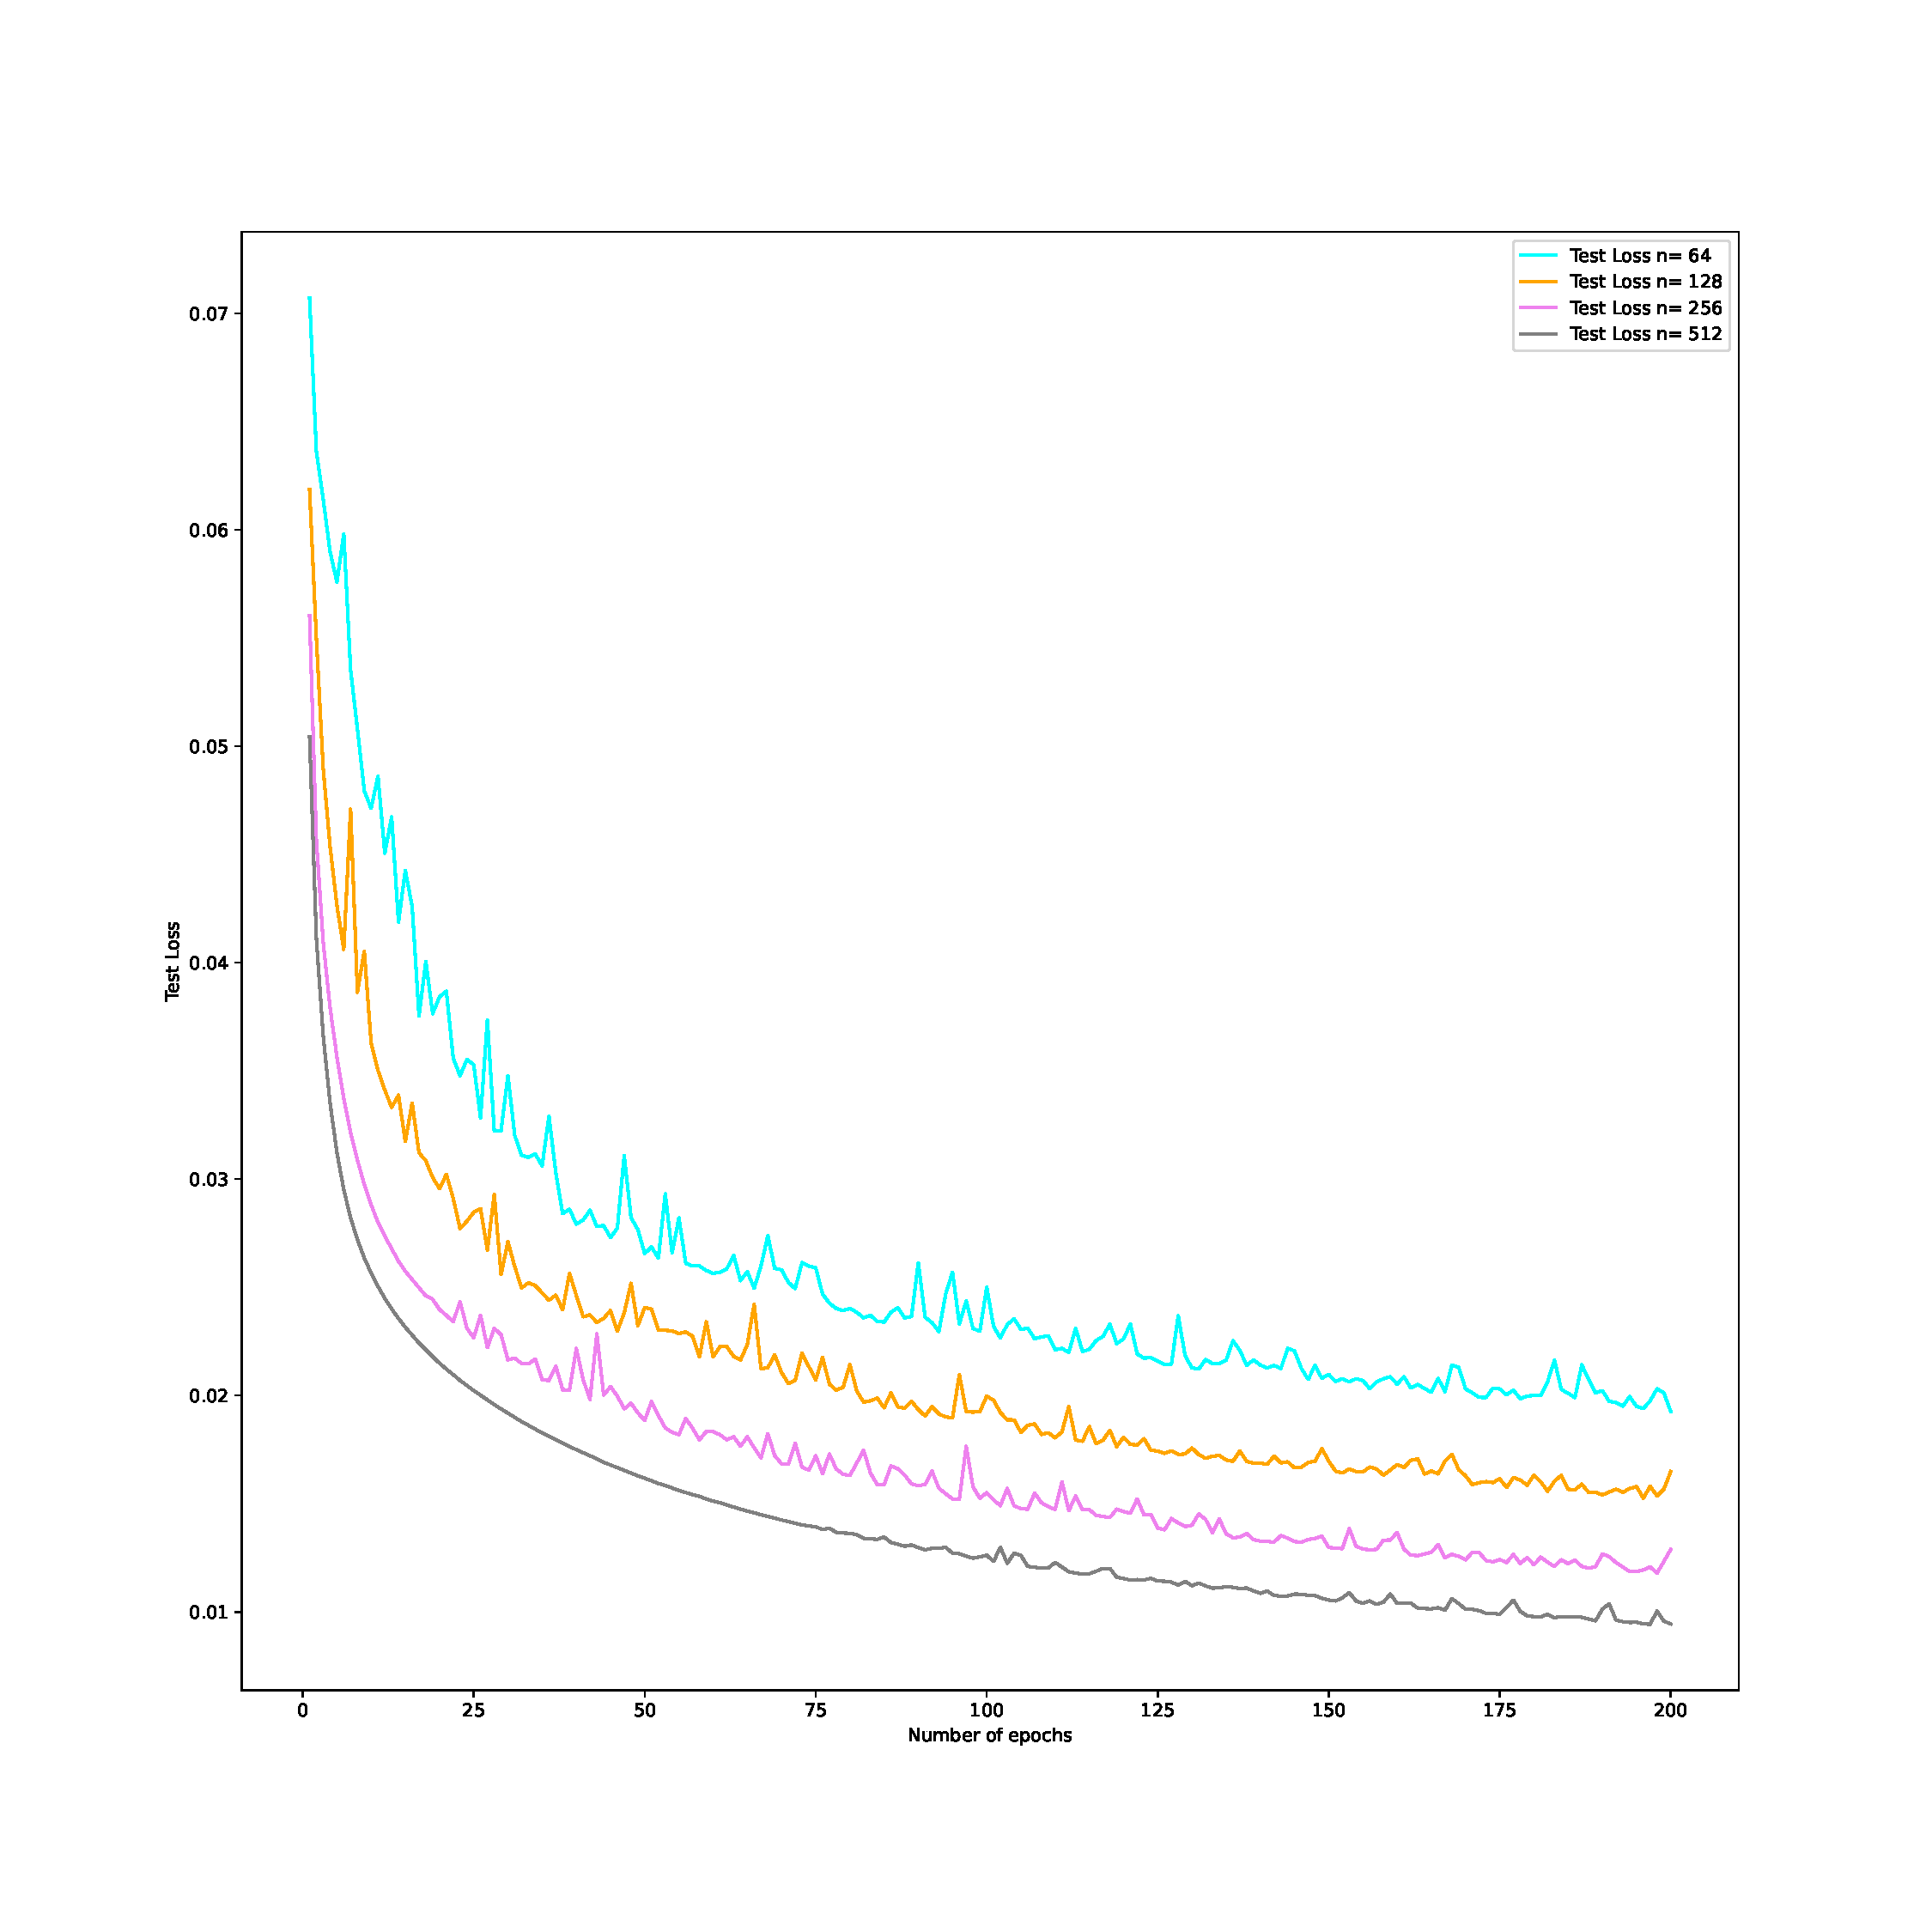
\includegraphics[scale=0.20]{Test Loss.pdf}
\end{center}


Los mejores resultados de las reconstrucciones de imágenes se obtuvieron con una tasa de aprendizaje igual a $1$ para todos los tamaños de capas intermedias. Las imágenes de la primer fila son las predicciones que arroja el modelo sobre el conjunto de testeo y la segunda fila son las imágenes originales del conjunto de datos de entrenamiento.

\begin{center}
\textbf{Figura N°6: \\ Reconstrucción de imágenes para $n=64$}
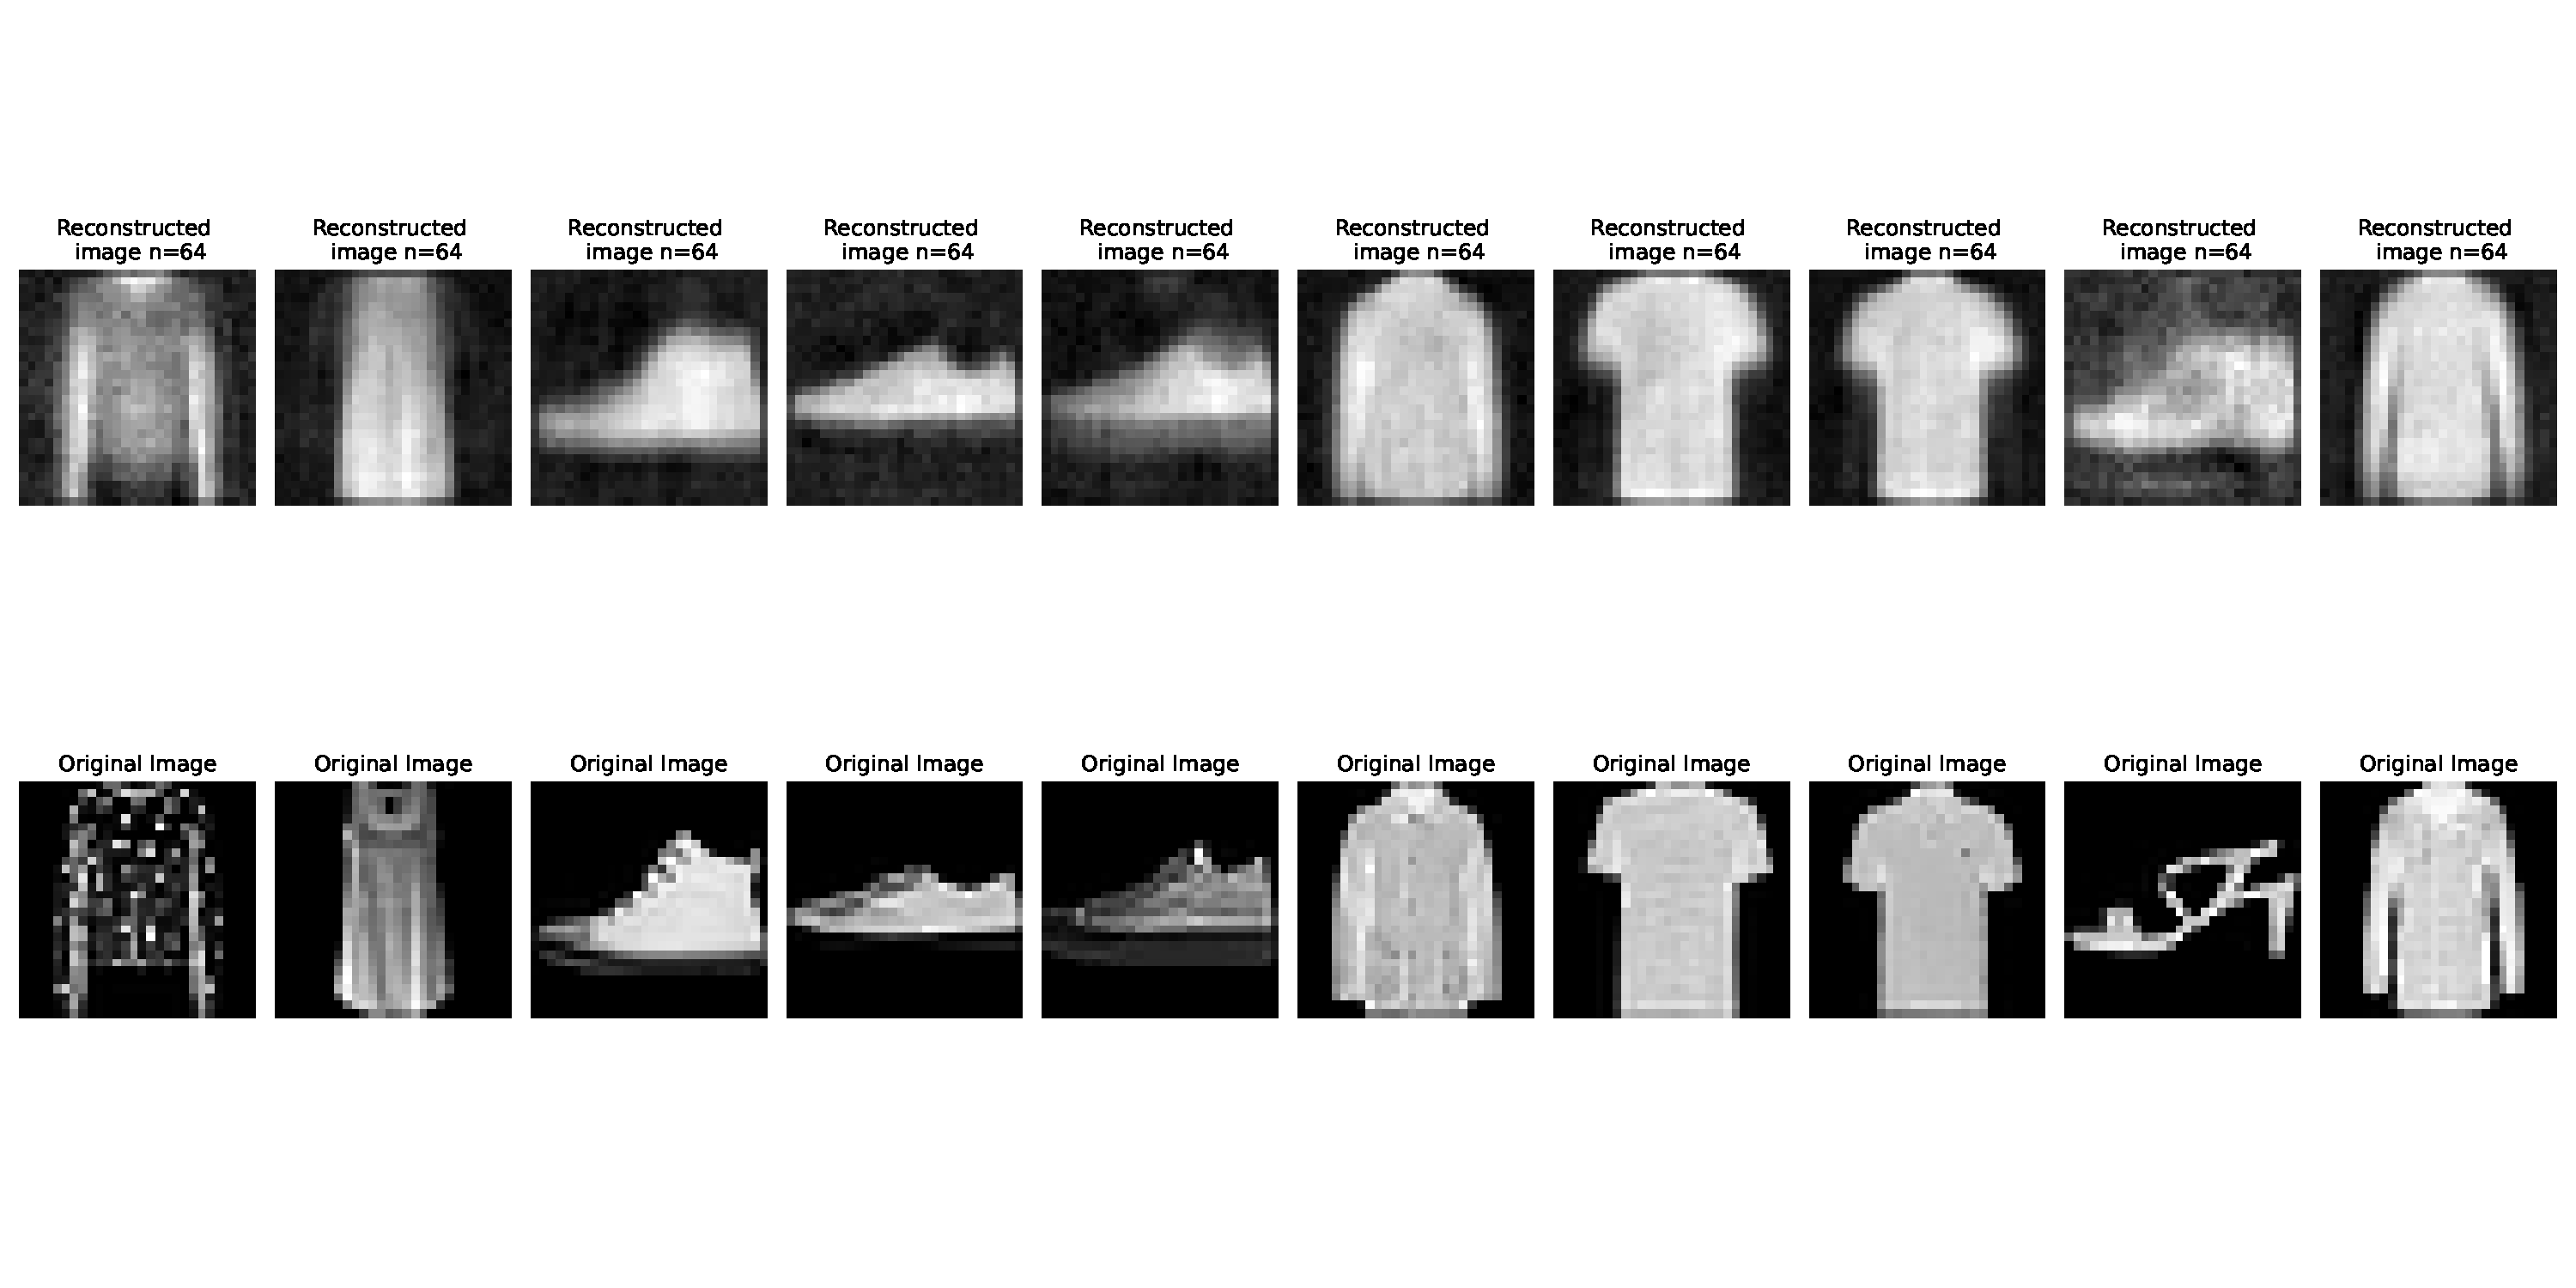
\includegraphics[scale=0.16]{Img64.pdf}
\end{center}

Al considerar una capa intermedia de 64 neuronas, todas ellas tienen que simular la información y encontrar patrones o relaciones de 784 neuronas, por lo que se pierde bastante información al comprimir los datos entre esas magnitudes. Sin embargo se nota que predice bastante bien las imágenes, sin confudirse entre prendas exceptuando por el primer vestido que se parece un pantalón y la sandalia que parece una zapatilla. No obstante, no se logran reconstrucciones muy nítidas de las imágenes originales.

\begin{center}
\textbf{Figura N°7: \\ Reconstrucción de imágenes para $n=128$}
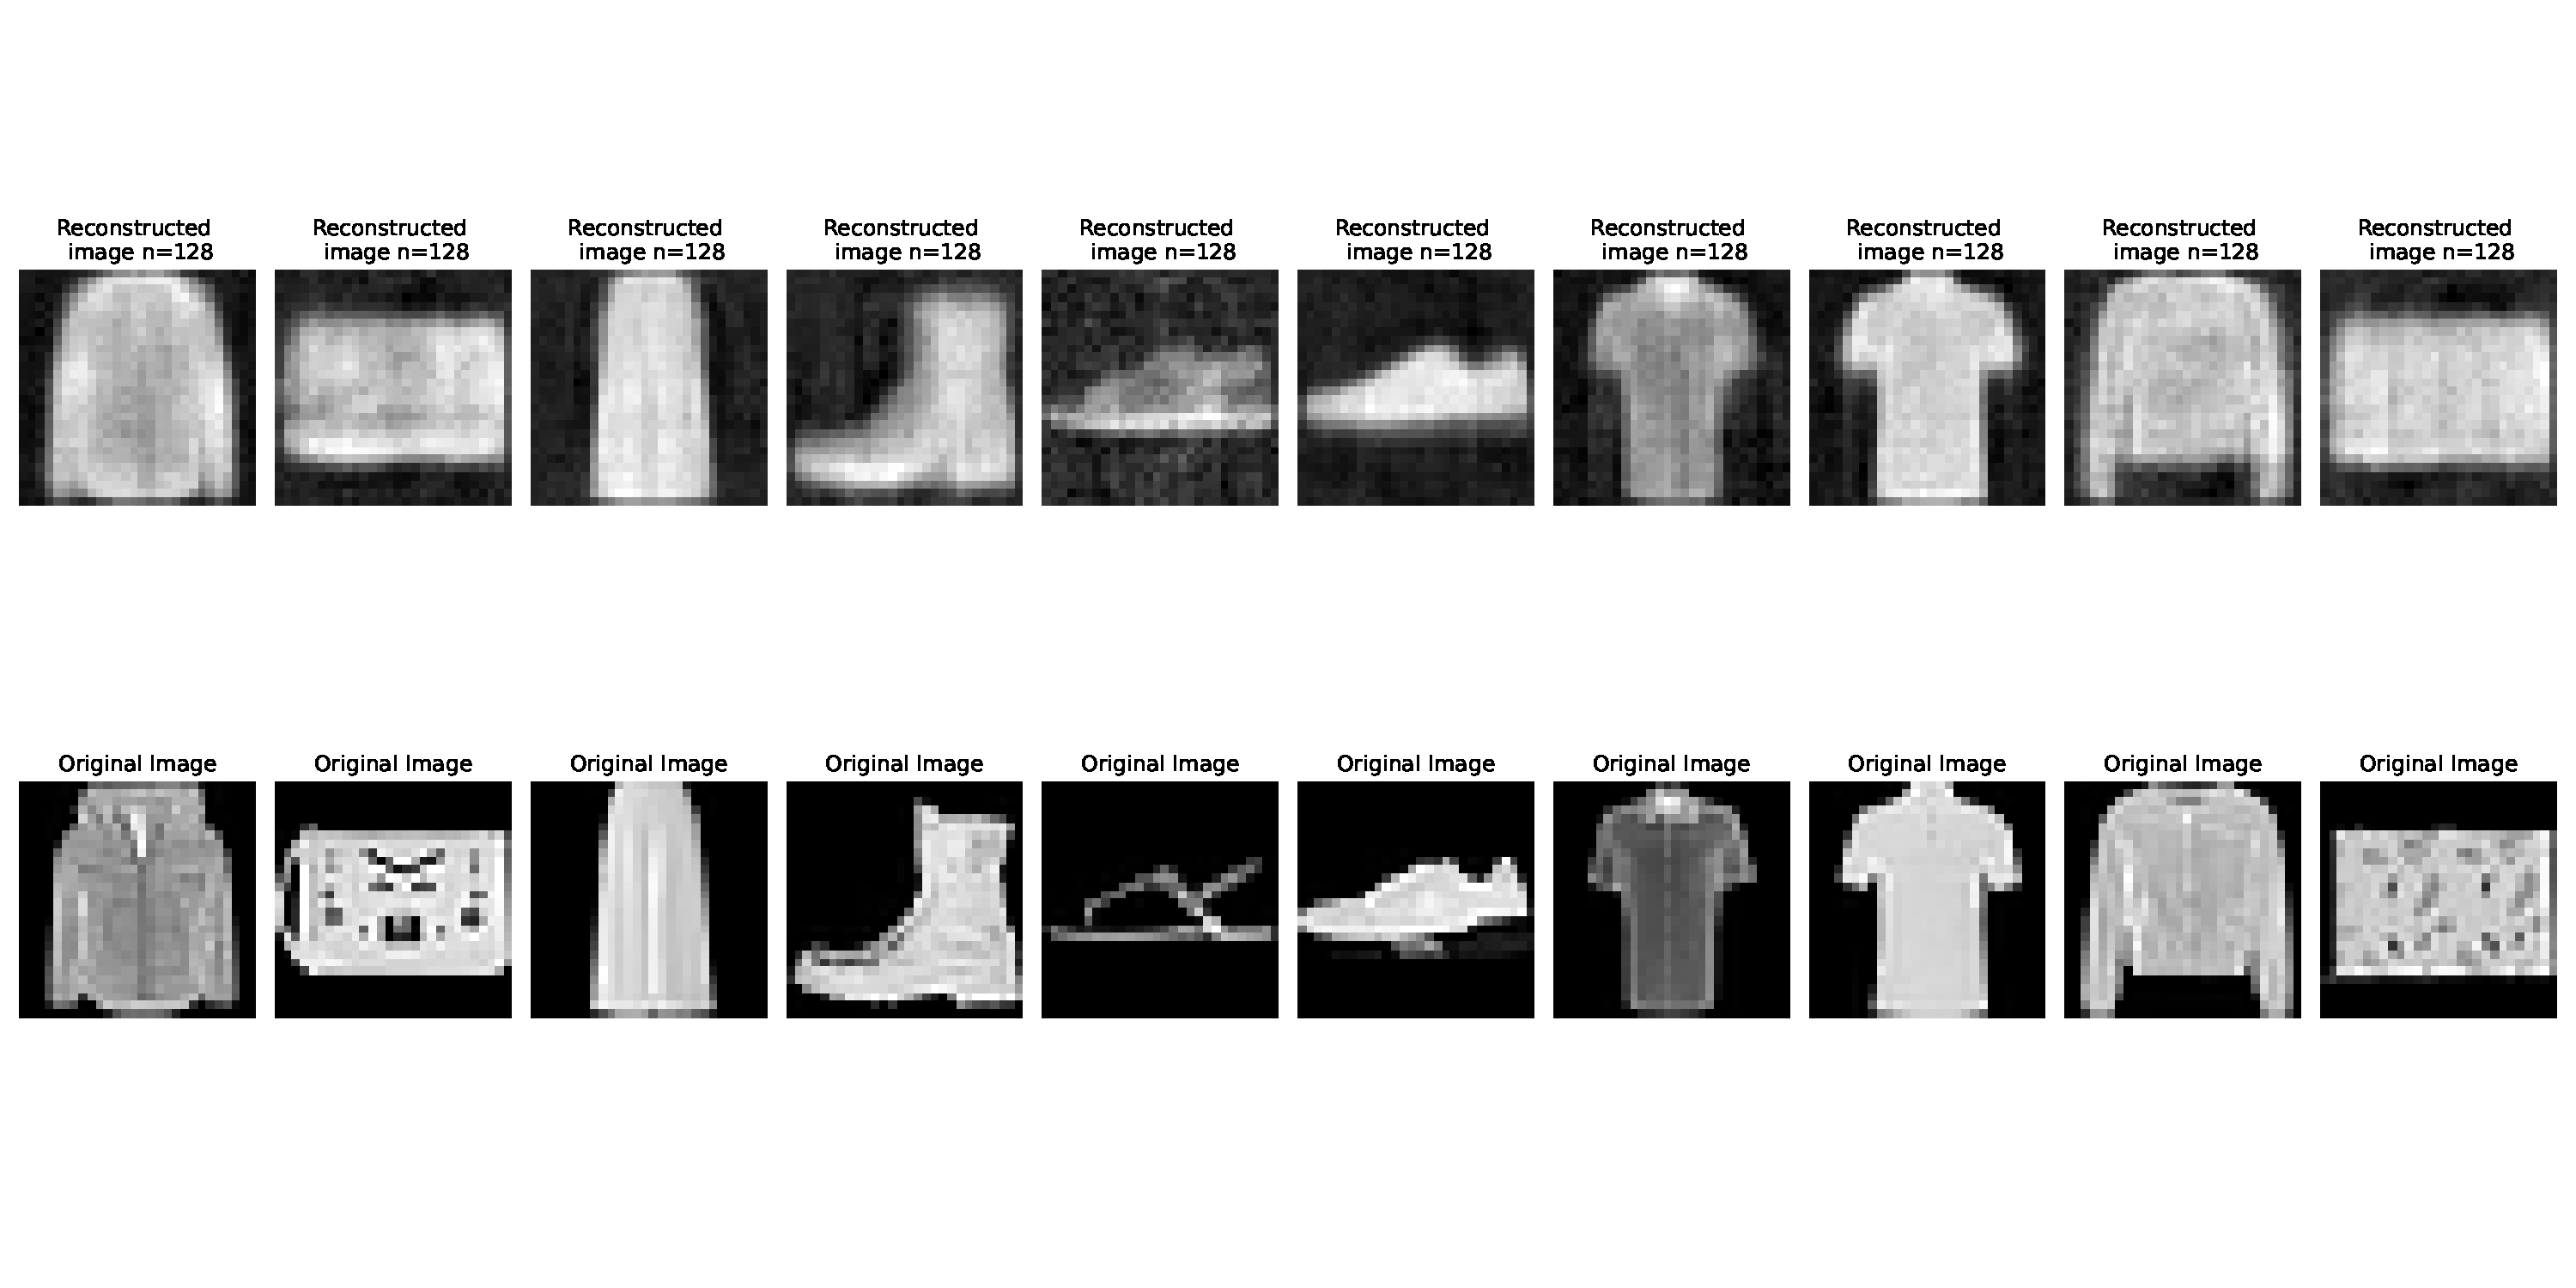
\includegraphics[scale=0.16]{Img128.pdf}
\end{center}



Cuando se establece una capa intermedia de 128 los resultados siguen siendo satisfactorios en general, teniendo algunas dificultades con predecir bien las sandalias, al igual que el caso anterior. 

\begin{center}
\textbf{Figura N°8: \\ Reconstrucción de imágenes para $n=256$}
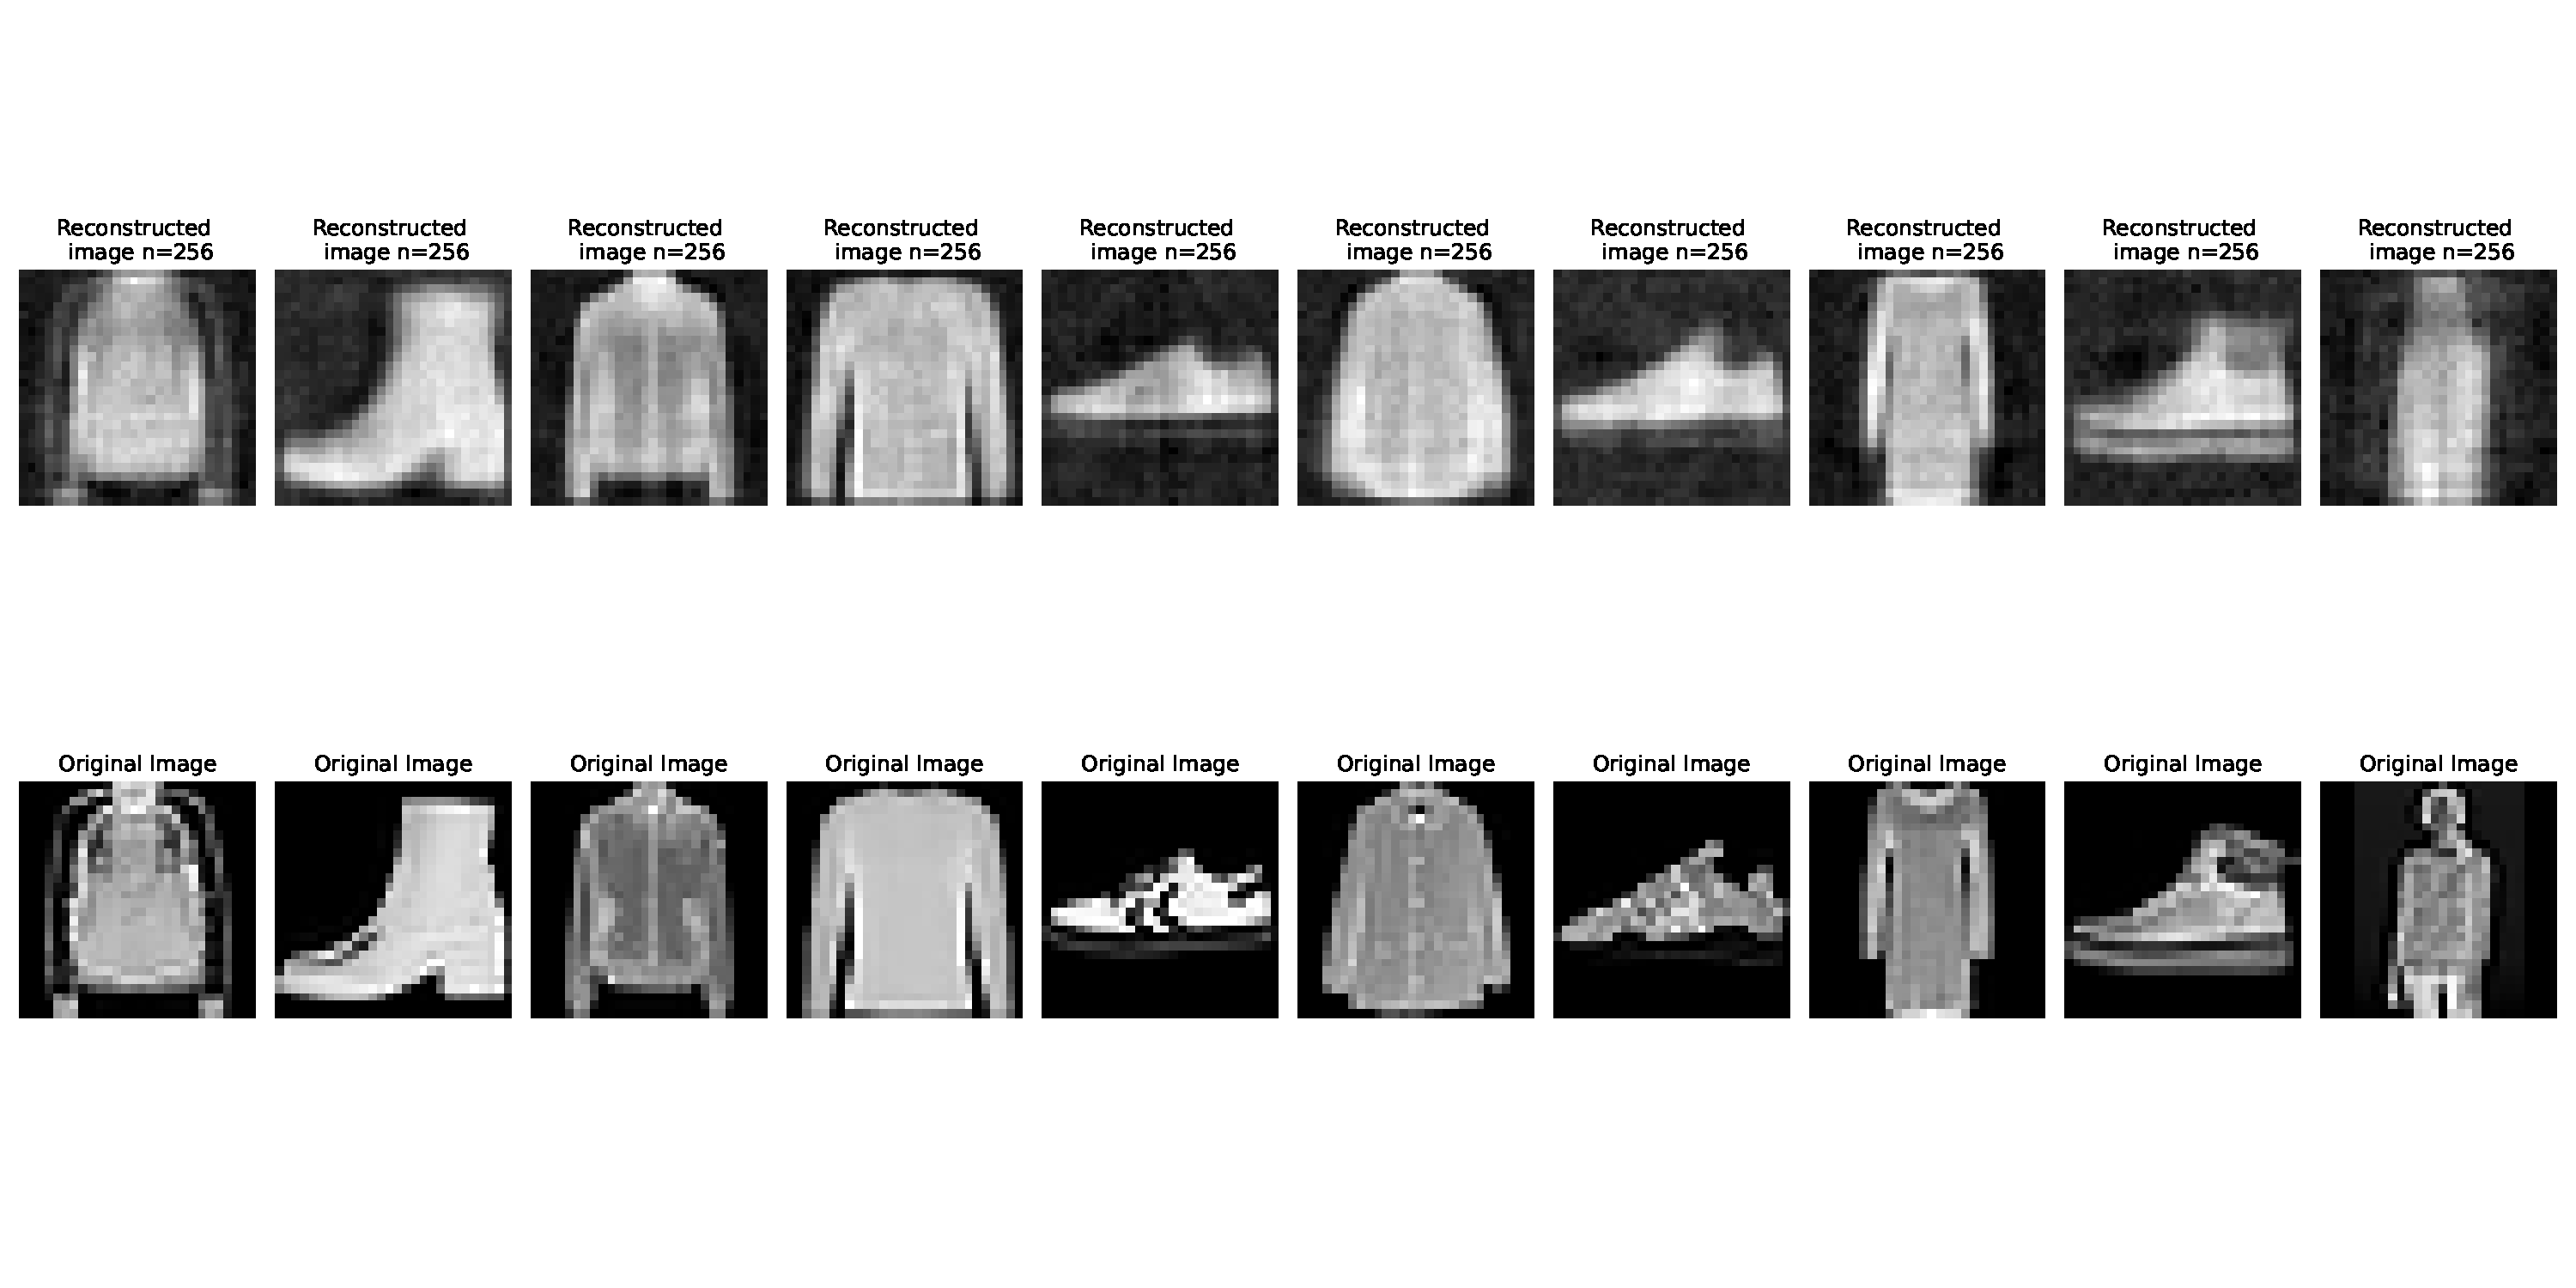
\includegraphics[scale=0.16]{Img256.pdf}
\end{center}

Con un tamaño de capa intermedia igual a 256 se siguen visualizando buenos resultados en general, notándose una mejora en la predicción de los vestidos.
\vspace*{5cm}
\begin{center}
\textbf{Figura N°9: \\ Reconstrucción de imágenes para $n=512$}
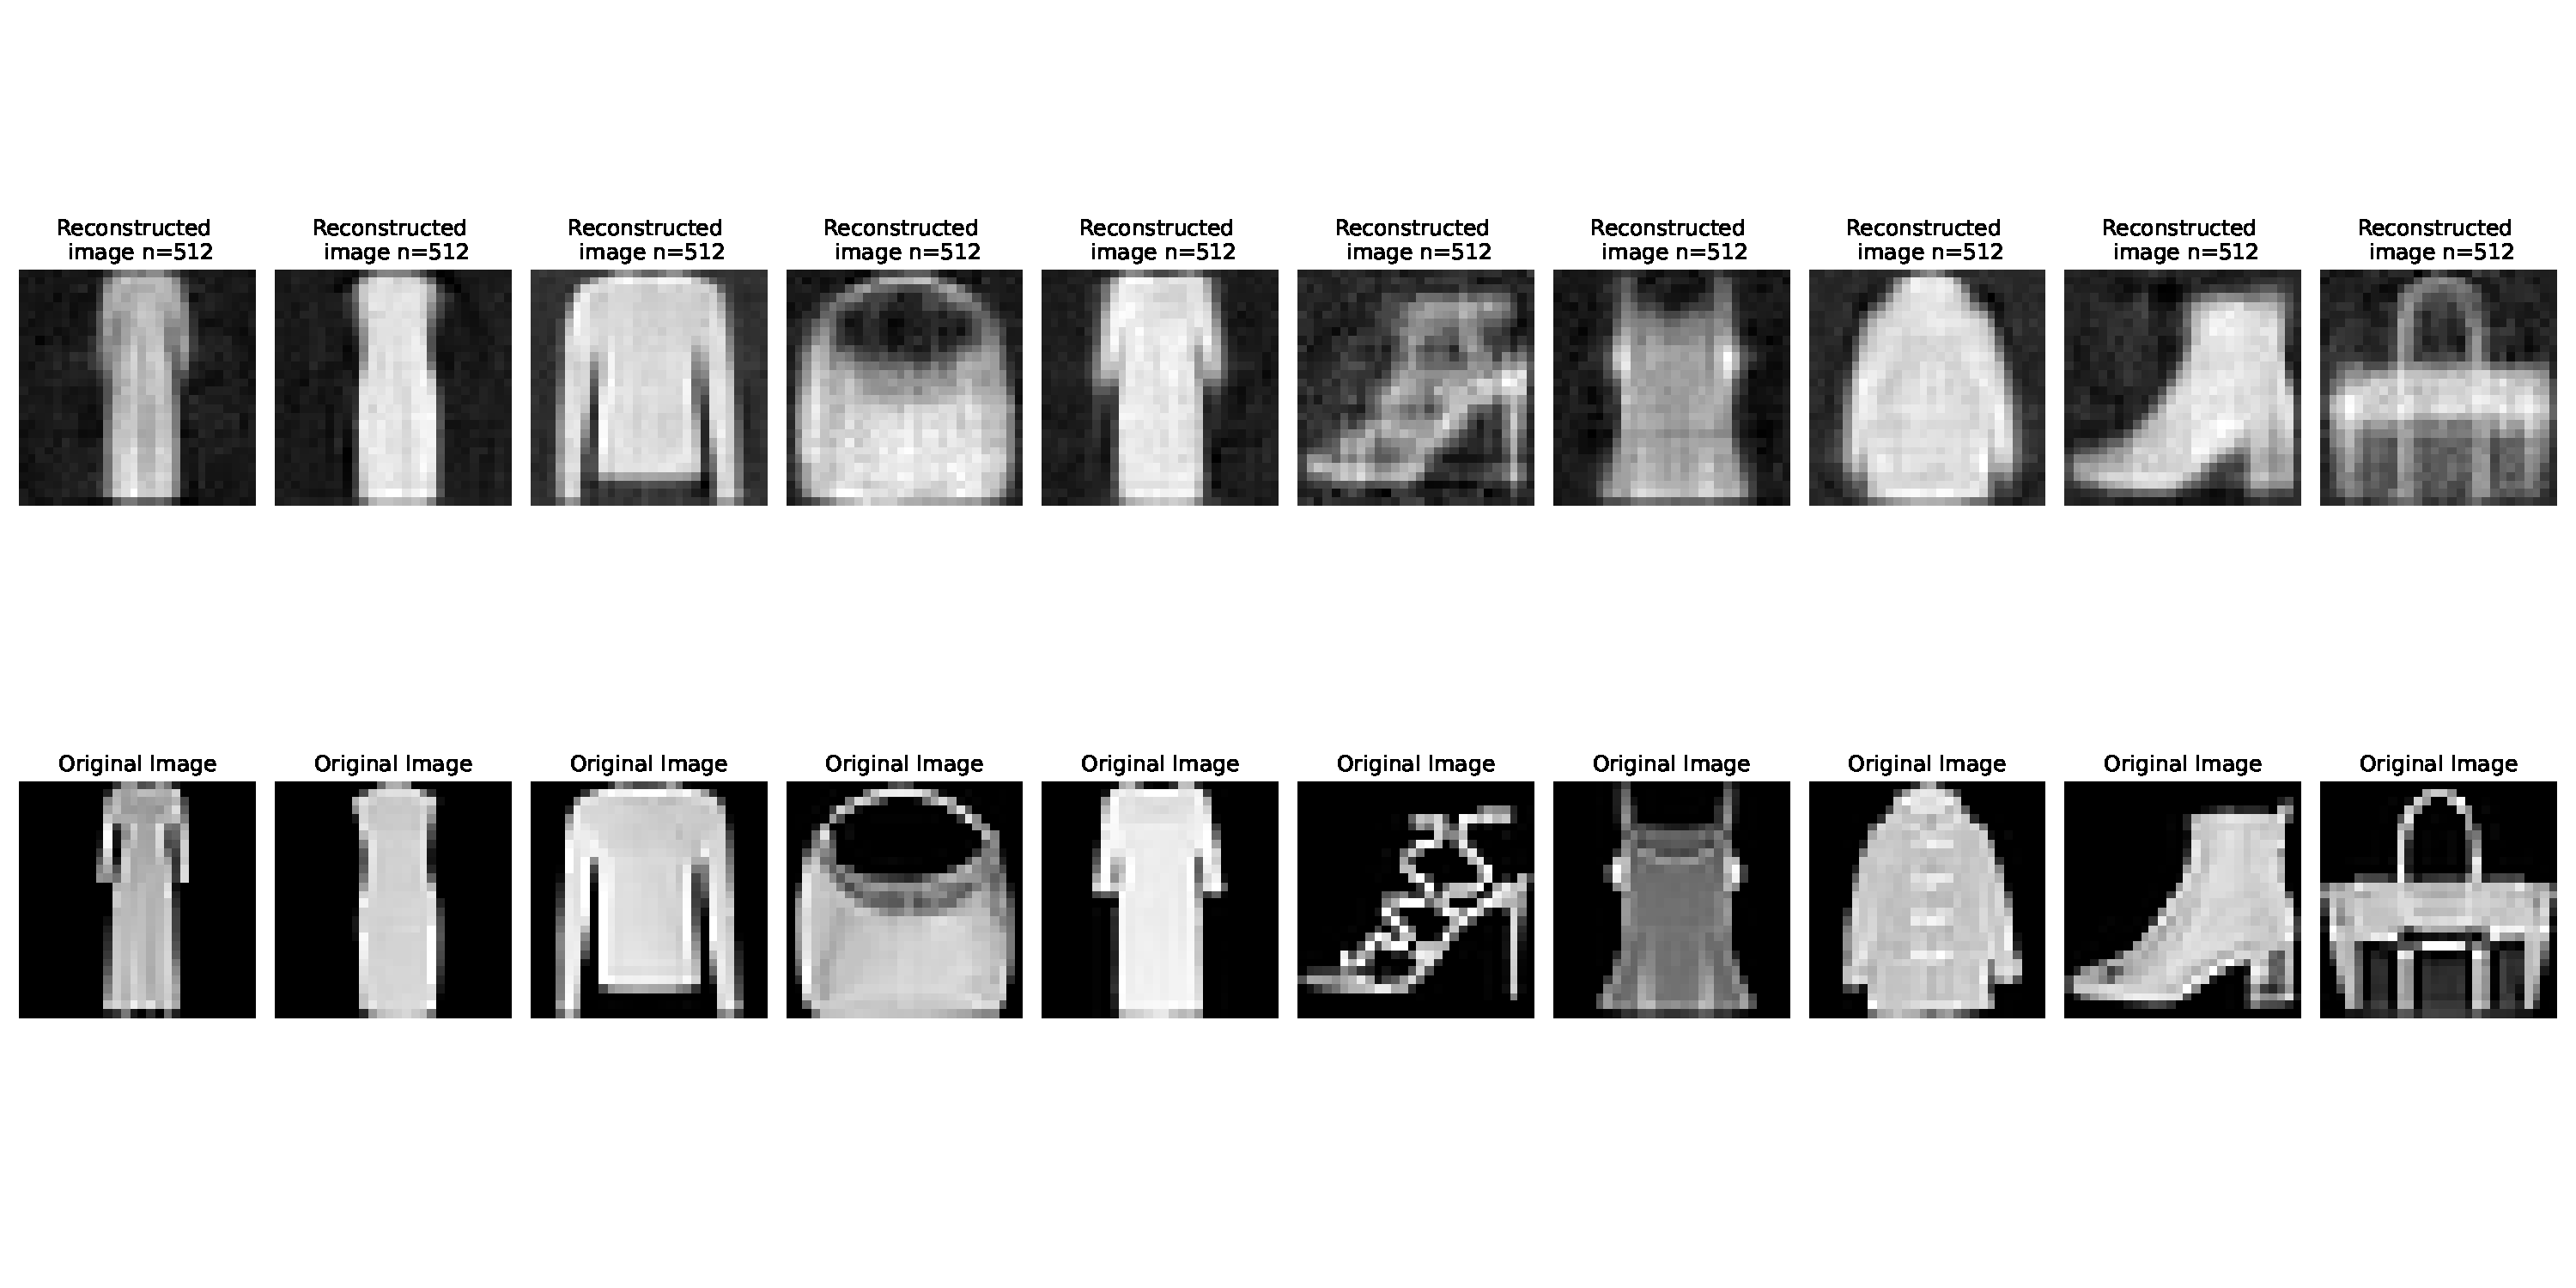
\includegraphics[scale=0.16]{Img512.pdf}
\end{center}

En la \textbf{Figura N°9} vemos que la reconstrucción mejora y la predicción también, en este último caso no se confunde en ninguna de las 10 prendas que se muestan. Los zapatos, zapatillas y sandalias eran las figuras que más le costaba diferenciar entre sí, no obstante, con una tamaño de capa intermedia igual a $512$ se nota que logra establecer una buena distinción entre ellos, además de no confundirse los vestidos con pantalones.

\begin{center}
\begin{large}
\textbf{Conclusiones}
\end{large}
\end{center}

Los resultados expuestos anteriormente demuestran que utilizar una \textit{red feed-forward autoencoder} con mini-batch de tamaño $1000$ e implementando el algoritmo del descenso por el gradiente estocástico a la función de error cuadático medio, es apropiado para la reconstrucción de las imágenes brindadas por el \textit{dataset Fashion MNIST}. A medida que aumenta el tamaño de la capa intermedia la predicción mejora bastante mientras que la reconstrucción de las imágenes sigue dejando algo que desear.  

Los mejores resultados se presentan cuando la capa intermedia es $n=512$ , esto lo podemos comprobar no solo con la visualización las imágenes anteriores sino también en los gráficos de las funciones de pérdida, donde las funciones correspondientes a dicho modelo son las que asumen los menores valores.

\end{multicols}
\end{document}
